\documentclass[a4paper,twoside]{article}
\usepackage{blindtext}  
\usepackage{geometry}

% Chinese support
\usepackage[UTF8, scheme = plain]{ctex}

% Page margin layout
\geometry{left=2.3cm,right=2cm,top=2.5cm,bottom=2.0cm}


\usepackage{listings}
\usepackage{xcolor}
\usepackage{geometry}
\usepackage{amsmath}
\usepackage{float}
\usepackage{hyperref}

\usepackage{graphics}
\usepackage{graphicx}
\usepackage{epsfig}
\usepackage{float}
\usepackage{wrapfig}

\usepackage{algorithm}
\usepackage[noend]{algpseudocode}

\usepackage{booktabs}
\usepackage{threeparttable}
\usepackage{longtable}
\usepackage{listings}
\usepackage{tikz}
\usepackage{multicol}

\usepackage{caption}
\usepackage{subcaption}

% cite package, to clean up citations in the main text. Do not remove.
\usepackage{cite}

\usepackage{color,xcolor}

%% The amssymb package provides various useful mathematical symbols
\usepackage{amssymb}
%% The amsthm package provides extended theorem environments
\usepackage{amsthm}
\usepackage{amsfonts}
\usepackage{enumerate}
\usepackage{enumitem}
\usepackage{listings}

\usepackage{textcomp}

\usepackage{indentfirst}
\setlength{\parindent}{2em} % Make two letter space in the first paragraph
\usepackage{setspace}
\linespread{1.5} % Line spacing setting
\usepackage{siunitx}
\setlength{\parskip}{0.5em} % Paragraph spacing setting

% \usepackage[contents =22920202204622, scale = 10, color = black, angle = 50, opacity = .10]{background}

\renewcommand{\figurename}{图}
\renewcommand{\lstlistingname}{代码} 
\renewcommand{\tablename}{表格}
\renewcommand{\contentsname}{目录}
\floatname{algorithm}{算法}

\graphicspath{ {images/} }

%%%%%%%%%%%%%
\newcommand{\StudentNumber}{22920202204622}  % Fill your student number here
\newcommand{\StudentName}{熊恪峥}  % Replace your name here
\newcommand{\PaperTitle}{实验(四) Shell程序设计和改进}  % Change your paper title here
\newcommand{\PaperType}{Unix程序设计} % Replace the type of your report here
\newcommand{\Date}{2022年11月4日}
\newcommand{\College}{信息学院}
\newcommand{\CourseName}{Unix程序设计}
%%%%%%%%%%%%%

%% Page header and footer setting
\usepackage{fancyhdr}
\usepackage{lastpage}
\pagestyle{fancy}
\fancyhf{}
% This requires the document to be twoside
\fancyhead[LO]{\texttt{\StudentName }}
\fancyhead[LE]{\texttt{\StudentNumber}}
\fancyhead[C]{\texttt{\PaperTitle }}
\fancyhead[R]{\texttt{第{\thepage}页,共\pageref*{LastPage}页}}


\title{\PaperTitle}
\author{\StudentName}
\date{\Date}

\lstset{
	basicstyle          =   \sffamily,          % 基本代码风格
	keywordstyle        =   \bfseries,          % 关键字风格
	commentstyle        =   \rmfamily\itshape,  % 注释的风格,斜体
	stringstyle         =   \ttfamily,  % 字符串风格
	flexiblecolumns,                % 别问为什么,加上这个
	numbers             =   left,   % 行号的位置在左边
	showspaces          =   false,  % 是否显示空格,显示了有点乱,所以不现实了
	numberstyle         =   \zihao{-5}\ttfamily,    % 行号的样式,小五号,tt等宽字体
	showstringspaces    =   false,
	captionpos          =   t,      % 这段代码的名字所呈现的位置,t指的是top上面
	frame               =   lrtb,   % 显示边框
}

\lstdefinestyle{PythonStyle}{
	language        =   Python, % 语言选Python
	basicstyle      =   \zihao{-5}\ttfamily,
	numberstyle     =   \zihao{-5}\ttfamily,
	keywordstyle    =   \color{blue},
	keywordstyle    =   [2] \color{teal},
	stringstyle     =   \color{magenta},
	commentstyle    =   \color{red}\ttfamily,
	breaklines      =   true,   % 自动换行,建议不要写太长的行
	columns         =   fixed,  % 如果不加这一句,字间距就不固定,很丑,必须加
	basewidth       =   0.5em,
}

\definecolor{keycolor}{RGB}{172, 42, 42}
\definecolor{mbleu}{RGB}{64,96,127}
\definecolor{vimvert}{RGB}{46, 139, 87}

\lstdefinestyle{MakefileBaseStyle}{
basicstyle=\ttfamily\scriptsize\color{black!90},%
stringstyle=\itshape\color{magenta},%
showstringspaces=false,%
keywordstyle=\bfseries\color{keycolor},%
commentstyle=\color{blue}\slshape,%
framexleftmargin=1mm,%
backgroundcolor=\color{black!2},%
}

\lstdefinestyle{MakefileStyle}{
	otherkeywords={.SUFFIXES},
	morekeywords={SUFFIX, CPP_,},
	moredelim=[is][\color{mbleu}]{/*}{*/},
	style=MakefileBaseStyle,%
	morecomment=[l][commentstyle]{\#},%
	emphstyle={\color{vimvert}},%
	moredelim=[s][\color{vimvert}]{\$(}{)}%
}

\lstdefinestyle{CppStyle}{
	language        =   c++,
	basicstyle      =   \zihao{-5}\ttfamily,
	numberstyle     =   \zihao{-5}\ttfamily,
	keywordstyle    =   \color{blue},
	keywordstyle    =   [2] \color{teal},
	stringstyle     =   \color{magenta},
	commentstyle    =   \color{red}\ttfamily,
	breaklines      =   true,   % 自动换行,建议不要写太长的行
	columns         =   fixed,  % 如果不加这一句,字间距就不固定,很丑,必须加
	basewidth       =   0.5em,
}

\algnewcommand\algorithmicinput{\textbf{Input:}}
\algnewcommand\algorithmicoutput{\textbf{Output:}}
\algnewcommand\Input{\item[\algorithmicinput]}%
\algnewcommand\Output{\item[\algorithmicoutput]}%

\usetikzlibrary{positioning, shapes.geometric}

% 流程图定义基本形状
\tikzstyle{startstop} = [rectangle, rounded corners, minimum width = 2cm, minimum height=1cm,text centered, draw = black]
\tikzstyle{io} = [trapezium, trapezium left angle=70, trapezium right angle=110, minimum width=2cm, minimum height=1cm, text centered, draw=black]
\tikzstyle{process} = [rectangle, minimum width=3cm, minimum height=1cm, text centered, draw=black]
\tikzstyle{decision} = [diamond, aspect = 3, text centered, draw=black]
% 箭头形式
\tikzstyle{arrow} = [->,>=stealth]

\newtheorem{assumption}{Assumption}[section]

\begin{document}
	
%%%%%%%%%%%%%%%%%%%%%%%%%%%%%%%%%%%%%%%%%%%%
\makeatletter % change default title style
\renewcommand*\maketitle{%
	\begin{center} 
		\bfseries  % title 
		{\LARGE \@title \par}  % LARGE typesetting
		\vskip 1em  %  margin 1em
		{\global\let\author\@empty}  % no author information
		{\global\let\date\@empty}  % no date
		\thispagestyle{empty}   %  empty page style
	\end{center}%
	\setcounter{footnote}{0}%
}
\makeatother
%%%%%%%%%%%%%%%%%%%%%%%%%%%%%%%%%%%%%%%%%%%%
	
	
\thispagestyle{empty}

\vspace*{1cm}

\begin{figure}[h]
	\centering
	
\includegraphics[width=4.0cm]{logo.png}
\end{figure}

\vspace*{1cm}

\begin{center}
	\Huge{\textbf{\PaperType}}
	
	\Large{\PaperTitle}
\end{center}

\vspace*{1cm}

\begin{table}[h]
	\centering	
	\begin{Large}
		\renewcommand{\arraystretch}{1.5}
		\begin{tabular}{p{3cm} p{5cm}<{\centering}}
			姓\qquad 名 & \StudentName  \\
			\hline
			学\qquad号 & \StudentNumber \\
			\hline
			日\qquad期 & \Date  \\
			\hline
			学\qquad院 & \College  \\
			\hline
			课程名称 & \CourseName  \\
			\hline
		\end{tabular}
	\end{Large}
\end{table}

\newpage

\title{
	\Large{\textcolor{black}{\PaperTitle}}
}
	
	
\maketitle
	
\tableofcontents
 
\newpage
\setcounter{page}{1}

\begin{spacing}{1.2}

\section{实验内容}

简单Shell的设计和实现。要求:

\begin{enumerate}
    \item 除了系统调用execve,不允许使用其他的exec函数。输入应当允许带多个参数(一行内可以表示),不考虑通配符 (即“*”、“?”、“-”等等)的处理。
    \item 输入错误命令能提示出错并进入下一轮接收命令状态。
    \item 可以用Ctrl-C和Ctrl-$\backslash$ 结束简单Shell的运行。
    \item 程序运行正确,提示简洁明确。
\end{enumerate}

\section{最简单的Shell实现}

实现一个最简单的Shell只需要三步:首先从标准输入流中读入一整行数据并利用空格拆分,然后\texttt{fork}当前进程,最后用\texttt{execve}执行命令。最后使用\texttt{waitpid}等待子进程结束,然后再次读入命令。

\subsection{运行效果}

按这种思路实现的Shell运行结果如图~\ref{fig:minimal},它可以通过用完整的绝对路径运行简单的Shell命令。
\begin{figure}[htb]
	\centering
	\caption{最简单的Shell}
	\label{fig:minimal}
	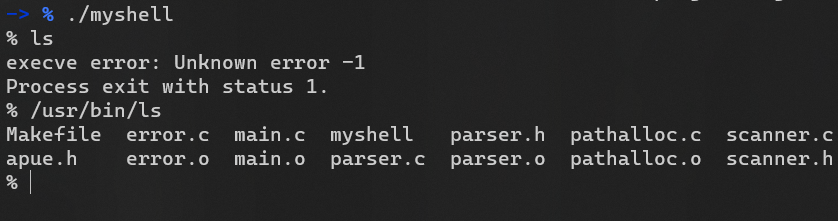
\includegraphics[width=0.6\textwidth]{minimal.png}
\end{figure}
并且能够正确地传递命令行参数。

\subsection{有什么问题}

今天,当用户使用Shell的时候所期待的重要的功能并不是简单地运行相应的程序。而是看重Shell可以通过许多便利的高级功能实现对简单程序的组合,
来方便一次完成批量、重复的操作。这是当今CLI相对GUI而言最主要的优点。显然,这些功能并不是简单地用空格拆分输入的命令就可以实现的。
因此需要更进一步地设计处理输入的命令的流程。

例如合法的Shell表达式\eqref{eq:shell_exp},
\begin{equation}
	\label{eq:shell_exp}
grep \ ab \ < \ test.txt \ | \ grep \ abc
\end{equation}
这条表达式先在文件test.txt中查找包含ab的行,然后再在这些行中查找包含abc的行。这个表达式中使用了管道符“\textbar”和I/O重定向符。
为了正确处理这条Shell表达式,直接用空格拆分输入的命令是不够的。因为管道符和I/O重定向符的存在,对一条命令的处理不只是简单的从左向右
依次扫描,而需要对输入的命令进行更进一步分析,首先执行管道符左边的命令,执行时进行I/O重定向,然后将标准输出的结果为输入传递给管道符右边的命令。
再比如,Shell表达式\eqref{eq:shell_exp2},
\begin{equation}
	\label{eq:shell_exp2}
wget \ <some \ url> \ | \ grep \ error > log.txt \ \&
\end{equation}
这条表达式中使用了后台运行符“\&”,这个符号的作用是要求Shell启动程序后立刻返回为下一条指令就绪,而将命令放到后台运行,而不是等待命令执行完毕后再执行下一条命令。
这个符号的效果对整条表达式起效,而非最后一部分的\texttt{grep}。这样一来,空格拆分、从左往右的处理方式就不再适用,否则会给出错误的结果。

因此,\emph{当管道、I/O重定向、后台执行等功能嵌套混合使用时,Shell需要具有更强的对输入命令的分析能力,来处理不同表达式中存在的结合性和优先级。}

\section{改进的Shell设计}

\subsection{设计目标}

为了改进Shell的设计,需要先定下合理的目标,因为现代Shell是一个极其复杂的系统,因此只能实现其中功能的一个子集。在这些功能中,最基础的是

\begin{itemize}
	\item 支持管道的处理
	\item 支持I/O重定向的处理
	\item 支持用括号等符号改变运行顺序
	\item 支持Shell脚本语句结束的分号;的处理
	\item 支持后台运行符号$\&$的处理
\end{itemize}

有了对这些功能的正确处理,就能实现绝大多数Shell所具有的、重要的基础功能。因此,这些功能是改进Shell设计的目标。而
为了这些功能的实现,需要对输入的命令进行更进一步的分析,这个分析的过程需要进行词法分析、语法分析,然后形成一棵语法树,
最后再对这棵语法树进行遍历,并运行相应的操作。为了符合Shell的一般规律,还需要实现在$PATH$环境变量中查找命令的功能。

\section{词法分析}

\subsection{词法分析的基本思想}

Shell的用户输入是一个字符串。为了有效地处理,我们首先需要将其拆分成最小有意义的字符串单元,这些字符单元具有被赋予、能被识别的意义。
这称之为一个Token,这个过程称之为词法分析\cite{aho2007compilers}。一个Token由名称和可选的Token值构成。在常见的编程语言中,Token包括标识符、运算符、关键字、字面量、分隔符等。
在我们需要支持的Shell命令词法分析中,我们只需要支持标识符、分隔符(;、(、))和运算符(\textbar、\textgreater、\textless)。

例如表达式\eqref{eq:shell_exp}经过词法分析,就会变成Token序列\eqref{eq:shell_token}。

\begin{multline}
	\label{eq:shell_token}
	[ (identifier,grep),(identifier,ab),(operator,<),(identifier,test.txt), \\ (operator,|),(identifier,grep),(identifier,abc) ]
\end{multline}

为了消除歧义,这里采用最长匹配的消歧义原则。即,当遇到一个Token的前缀是另一个Token的前缀时,选择最长的那个Token。

\subsection{词法分析的实现}

词法分析的实现代码见\nameref{sec:code}中的代码~\ref{code:scanner}。其中第一个参数是所需要词法分析的字符串的开头指针,
也用于返回获取一个Token以后的位置;第二个参数是其结尾指针;
后两个参数用于返回Token的开头和结尾位置。返回值代表Token类型,其中返回值若是字符'a'就代表终结符IDENTIFIER。
该函数的执行结果就是从命令中取出一个Token。


\section{语法分析}

得到了Token序列,需要正确地组织这些Token来形成符合Shell命令语义的抽象语法树(AST)。这个过程需要语法分析\cite{aho2007compilers}。
要进行语法分析,首先需要形式地定义Shell命令的语法规则,这种定义需要上下文无关语法。

\subsection{上下文无关语法}

上下文无关文法(CFG)是一种形式化的语法定义方法,它定义了一种语言的语法规则。上下文无关文法由四元组\eqref{eqn:cfg}定义。
\begin{equation}
	\label{eqn:cfg}
	G=(\mathcal{V},\Sigma,\mathcal{R},\mathcal{S})
\end{equation}
其中,$\mathcal{V}$是非终结符的集合,$\Sigma$是终结符的集合,$\mathcal{R}$是从$\mathcal{V}$到$(\mathcal{V} \cup \Sigma)^*$的关系,使得$\exists \omega \in (\mathcal{V}\cup \Sigma)^*: (S,\omega)\in \mathcal{R}$,$\mathcal{S}$是开始符号。

上下文无关文法具有足够强的表达力来表达大多数编程语言的语法规则。而巴克斯-诺尔范式(BNF)是上下文无关文法的一种常用表示。
在Shell命令的语法分析中,我们需要通过CFG定义的是Shell命令的语法规则。根据我们需要支持的内容,我们需要支持括号表达式、重定向、管道等几种
二元表达式、后台运行$\&$和行结束;等几种一元表达式,因此可以定义\eqref{eq:shell_cfg}的CFG。
\begin{equation}
	\label{eq:shell_cfg}
	\begin{aligned}
		command &\rightarrow (line)^* \\
		line &\rightarrow pipe \operatorname{|} back  \operatorname{|} list \\
		back &\rightarrow line \operatorname{'\&'} \\
		list &\rightarrow list \operatorname{';'} \\
		pipe &\rightarrow exec \operatorname{|} pipe \\ 
		exec &\rightarrow paren \operatorname{|} redirect \operatorname{|} IDENTIFIER (\operatorname{'-'}IDENTIFIER)^*\\
		paren &\rightarrow \operatorname{'('} redirect \operatorname{')'} \\
		redirect &\rightarrow exec (\operatorname{'>'}\operatorname{|}\operatorname{'>>'}) IDENTIFIER \operatorname{|} exec \operatorname{'<'} IDENTIFIER \\
	\end{aligned}	
\end{equation}
根据\eqref{eq:shell_cfg}的定义对表达式\eqref{eq:shell_exp}进行语法分析,得到的AST如图~\ref{fig:shell_ast}所示。

\begin{figure}[htb]
	\centering
	\caption{命令\eqref{eq:shell_exp}的AST}
	\label{fig:shell_ast}
	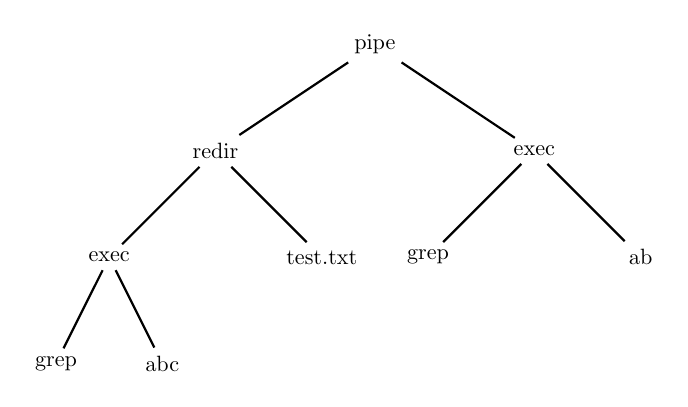
\begin{tikzpicture}[thick,scale=0.9, every node/.style={scale=0.8}]
		\node {pipe}
            child {node {redir}
                child {node {exec}
					child{node {grep}}
					child{node {abc}}
                }
                child [missing] {}
                child {node {test.txt}
                }
            }    
            child [missing] {} 
            child [missing] {}
            child { node {exec}
                child {node {grep}
                }
                child [missing] {}
                child {node {ab}
                }
            };
	\end{tikzpicture} 
\end{figure}

只要生成该AST,就可以对输入的命令进行解释执行了。因为Shell命令中我们支持的子集不需要语义分析。
为了生成正确的AST,需要使用递归下降法实现正确的Parser进行语法分析。

\subsection{递归下降法}

递归下降法是一种自上而下的语法分析方法,它的基本思想是:从文法的开始符号开始,逐步推导出输入串的语法结构。
递归下降法的实现需要使用递归函数,每个递归函数对应文法中的一个非终结符,每个递归函数的功能是:
从输入串中读取一个符号,判断该符号是否符合文法中对应的语法规则,
如果符合,则继续读取下一个符号,直到读取完整个输入串。如果输入串中的符号不符合文法中对应的语法规则,则报错。

本Shell的实现采用了语法制导的翻译(Syntax-directed Translation)。即整个语句的编译过程完全由Parser部分驱动。在运行
语法分析的过程中同时进行词法分析。而不是对不同阶段进行明确的区分。这样做的原因是所支持的Shell命令的语法规则比较简单,不需要
进行模块间非常明确的隔离就可以完成。同时,同时进行语法分析和语义分析有助于减少内存足迹(Memory Footprint),提高Shell运行
的效率。

在这一过程中,语法错误错误的命令输入会被发现,然后输出错误信息。而路径错误等语义上的错误会在运行时被发现。

本Shell的语法分析实现位于\texttt{parser.c}中,其中\texttt{parse\_line}函数对应文法中的\texttt{line}非终结符,以此类推。
具体见代码实现,或者\nameref{sec:code}中的代码~\ref{code:parser}。

\section{解释执行}

得到了抽象语法树,就可以对输入的命令进行解释执行了。
这个过程需要对抽象语法树进行遍历,然后对遍历到的节点进行相应的操作。这是对树状结构的深度优先遍历。
具体的过程在\texttt{main.c}的\texttt{run\_command}中,它判断\texttt{command\_t}中的类型
字段,然后转换成正确的结构体类型,最后对相应的表达式进行执行,执行时会对自身进行递归调用。

在这一阶段会通过\texttt{fork}创建子进程,在子进程中通过\texttt{execve}对相应的可执行文件进行执行。
由于处理\texttt{fork}返回值的过程固定而重复,并且在Shell中的处理就是输出报错信息并停止执行。所以
实现了\texttt{fork\_panic}函数来简化处理,其代码如代码~\ref*{code:forkpanic}。

\begin{lstlisting}[numbers=left,style=CppStyle,caption=解释执行,label={code:forkpanic}]
int fork_panic()
{
	int pid = fork();
	if (pid < 0)
	{
		err_exit(pid, "fork");
	}
	return pid;
}
\end{lstlisting}

\subsection{执行I/O重定向}

为了执行I/O重定向,就需要将标准输入输出的文件描述符重新打开到相应的文件中,如代码~\ref{code:ioredir}。

\begin{lstlisting}[numbers=left,style=CppStyle,caption=I/O重定向,label={code:ioredir}]
rcmd = (redir_command_t *)cmd;
fd = open(rcmd->file, rcmd->mode | O_SYNC | O_TRUNC);
if (fd < 0)
{
	err_exit(fd, "open %s failed\n", rcmd->file);
}
dup2(fd, rcmd->fd);
close(fd);
run_command(rcmd->cmd);
\end{lstlisting}


\subsection{执行管道}

管道是一种重要的Shell特性,它可以将一个命令的输出作为另一个命令的输入。一个进程在管道中写入的内容会被另一个
进程读取,实现了一种进程间通信机制。管道的实现需要使用\texttt{pipe}函数创建管道,然后使用\texttt{dup2}函数将管道的
读写端重定向到两个进程的标准输入输出上。因此我们创建两个子进程,进行相应的重定向,然后在两个子进程中分别递归调用来执行
\texttt{pipe} AST节点的左右两个操作数。
其实现片段如代码~\ref{code:pipe}。
在主进程中,我们也需要等待两个子进程的结束。

\begin{lstlisting}[numbers=left,style=CppStyle,caption=处理管道的执行,label={code:pipe}]
pcmd = (pipe_command_t *)cmd;
if (pipe(p) < 0)
{
	err_quit("pipe");
}
if ((pid1 = fork_panic()) == 0)
{
	dup2(p[1], STDOUT_FILENO);
	close(p[0]);
	close(p[1]);
	run_command(pcmd->left);
}
if ((pid2 = fork_panic()) == 0)
{
	dup2(p[0], STDIN_FILENO);
	close(p[0]);
	close(p[1]);
	run_command(pcmd->right);
}
close(p[0]);
close(p[1]);
waitpid(pid1, NULL, 0);
waitpid(pid2, NULL, 0);
\end{lstlisting}

\subsection{后台执行}

支持后台执行符号\texttt{\&},即在命令后面加上\texttt{\&},可以使命令在后台执行,而不会阻塞Shell的执行。
这一功能的实现相当简单。在执行之后不经过\texttt{wait}即返回,这样就不会阻塞Shell的执行。

其它解释执行阶段的具体实现见代码,或者\nameref{sec:code}中的代码~\ref{code:executor}。


\section{从环境变量$PATH$中查找程序}

在Shell中,我们可以直接输入程序名,而不需要输入程序的绝对路径,Shell会自动从环境变量$PATH$中查找程序。
这是Shell最重要的功能之一。为了实现这一功能,我们再进行\texttt{execve}前也必须进行查找。

本实现中查找$PATH$环境变量内容的函数为\texttt{find\_in\_path},其代码位于\texttt{findcmd.c}中,内容如
\nameref{sec:code}中的代码~\ref*{code:findpath}。它的实现原理非常简单。首先,Linux下的$PATH$环境变量都是以
冒号分隔的,所以我们可以通过\texttt{strtok}函数将其分割成多个字符串,然后利用上次实验中使用到的$path\_alloc$
函数分配路径的内存空间,最后将分割出来的字符串拼接到路径后面,然后用$fstat$判断该路径下是否存在该文件,如果存在则返回该路径。
这样查找到的就是首个匹配的文件。

\section{遇到的问题和解决方法}

在实现以上功能时,所遇到的问题就是I/O重定向不正常工作。

\subsection{I/O重定向不正常工作}

这个问题的来源是因为误以为\texttt{open}打开的文件描述符是会选择最小的可用的文件描述符,但是实际上
这种假设在一些内核版本中成立,而在一些内核中并不是这样的。因此,不能依赖先\texttt{close}相应的
标准输入输出文件流,然后再\texttt{open}文件,这样会导致文件描述符错误,使得I/O重定向失败。

正确的方式是调用\texttt{dup2}函数,将文件描述符复制到标准输入输出文件流的文件描述符,
然后关闭\texttt{open}返回的相应描述符。这样就可以保证文件描述符正确。

\section{运行效果}

\subsection{简单的命令}

运行简单的命令,如纯粹地运行某一程序、或者加入简单的参数的效果如图~\ref{fig:simple}所示。
\begin{figure}[htb]
	\centering
	\caption{简单的命令}
	\label{fig:simple}
	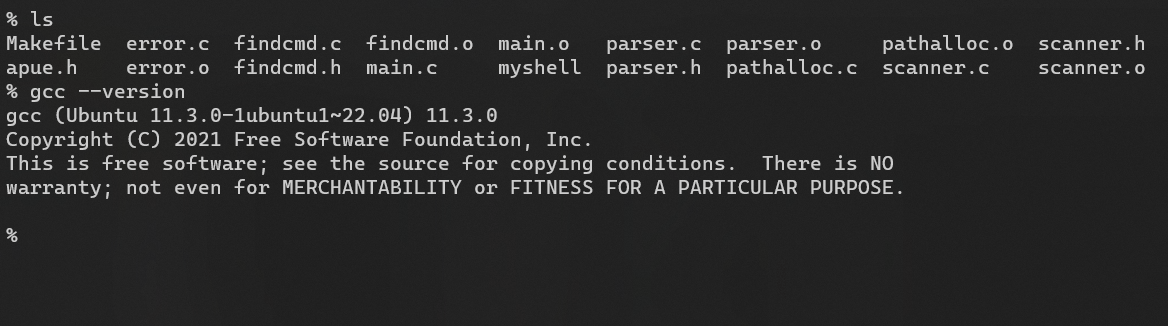
\includegraphics[width=0.8\textwidth]{simple.png}
\end{figure}
可见Shell能从$PATH$中查找到相应的程序,然后使得程序能够正常运行。命令行参数,
例如\texttt{--version}能够被正确解析然后传入\texttt{gcc}程序中。

\subsection{管道}

使用管道连接程序,从文本文件\texttt{test.txt}中读取内容,然后将先查找包含
\texttt{abc}的结果,再查找包含\texttt{ab}的结果,最后将结果输出到标准输出流中,
显示在终端上。这一功能可以使用管道符连接一个\texttt{cat}命令和两个\texttt{grep}命令完成。
实际的执行结果如图~\ref{fig:pipe}
\begin{figure}[htb]
	\centering
	\caption{Pipe}
	\label{fig:pipe}
	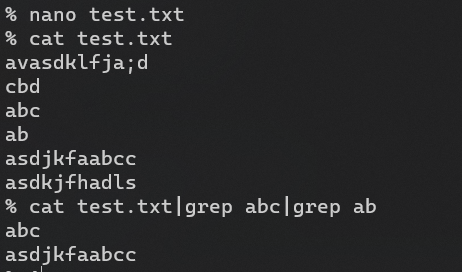
\includegraphics[width=0.4\textwidth]{pipe.png}
\end{figure}
可见,Shell能够正确地将管道符连接的命令的输入输出流连接起来,然后最右侧的\texttt{grep}输出了正确的结果。

\subsection{I/O重定向}

为了测试I/O重定向的功能,就需要测试对标准输入的重定向和对标准输出的重定向两个部分。我们首先将ls的结果重
定向到文件\texttt{dir.txt}中,然后再将\texttt{dir.txt}的内容定向到\texttt{grep}的输入中,在其中
查找串\texttt{error}。这样就可以测试I/O重定向的功能。实际的执行结果如图~\ref{fig:redirect_result}。
\begin{figure}[htb]
	\centering
	\caption{I/O重定向结果}
	\label{fig:redirect_result}
	\begin{subfigure}{0.4\textwidth}
		\centering
		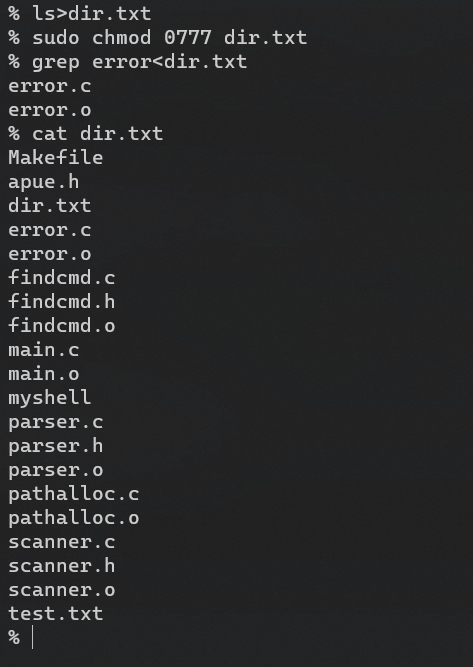
\includegraphics[width=\textwidth]{stdin.png}
		\caption{重定向标准输入}
		\label{fig:f2}
	\end{subfigure}
	\begin{subfigure}{0.4\textwidth}
		\centering
		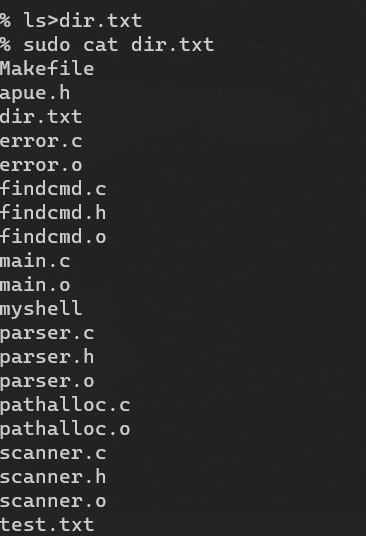
\includegraphics[width=\textwidth]{stdout.png}
		\caption{重定向标准输出}
		\label{fig:f3}
	\end{subfigure}
\end{figure}
可见,Shell能够正确地将标准输入重定向到文件中,然后将文件的内容作为标准输入传入\texttt{grep}程序中。
这表明I/O重定向的两个方向都被Shell正确地实现了。

\subsection{后台执行}

为了测试后台运行,我们使用\texttt{wget}命令对文件进行下载来模拟长时操作。然后使用\&符号将其放到后台执行。
运行结果如图~\ref{fig:background}所示。
\begin{figure}[htb]
	\centering
	\caption{后台执行}
	\label{fig:background}
	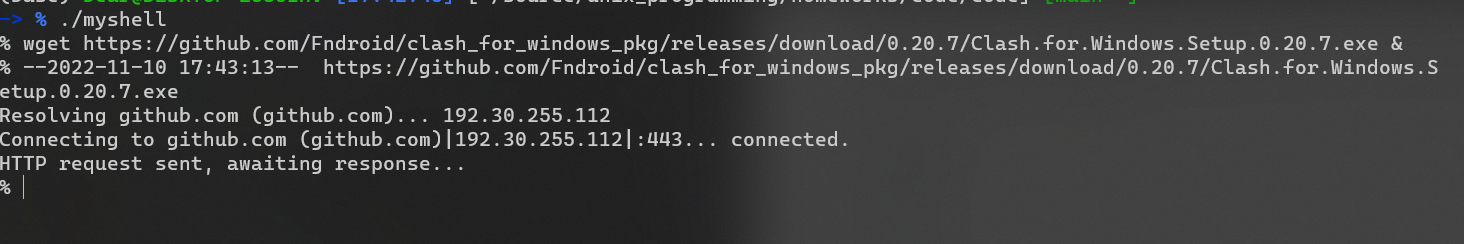
\includegraphics[width=0.4\textwidth]{back.png}
\end{figure}
可以发现,执行wget之后,Shell会立即返回,而不会等待wget的执行结果。这是出现了Shell提示符"\%"。
这表示后台执行的功能得到了正确的实现。

\section{软件工程上的处理}

为了对命令进行更好的解析处理,该Shell实现的代码规模相对较大。为了有效地进行管理,保证
可扩展性和可维护性,采用了一些措施。

\subsection{利用内存布局实现伪多态}

为了适应抽象语法树的节点有多个不同类型的特点,在设计抽象语法树的节点的数据结构时,可以通过指针类型转换的规则
模拟“类型擦除”来实现一定的多态能力。这一点在主要使用C语言的大型项目,例如Linux内核中得到了大量的应用。

这种方式主要的原理如图~\ref{fig:poly}所示。
\begin{figure}[ht]
	\centering
	\caption{AST节点结构}
	\label{fig:poly}
	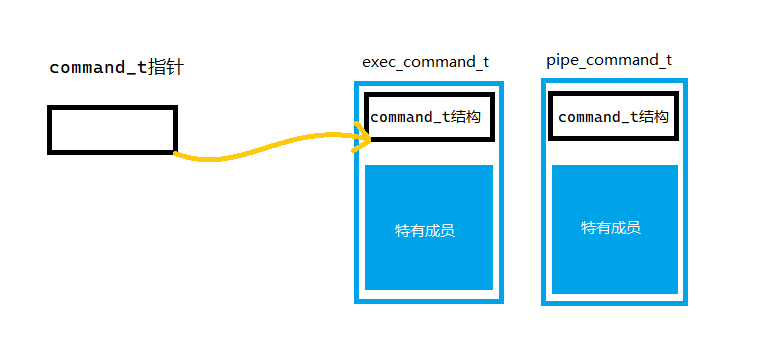
\includegraphics[width=0.6\textwidth]{poly.png}
\end{figure}
每一个AST节点中都具有一个\texttt{command\_t}类型的“头”结构,当我们传递一个AST节点的指针时,直接传递
\texttt{command\_t}类型的指针即可。在需要使用具体的AST节点类型时,可以通过其中的字段进行判断,
然后利用指针类型转换的规则\cite{iso1999iso}将\texttt{command\_t}转换成对应的具体类型。

这种方法在逻辑上实现了一种“is-a”的继承关系。这解决了缺乏面向对象程序设计能力的C语言当代码库的规模
扩大时面对大量类型不容易管理的问题。

\subsection{恰当分割文件}

为了保证代码的可读性,每个文件不宜太长\cite{martin2009clean}。因此在这个Shell实现中,将代码分割成了多个文件,每个文件
大致负责一个功能的实现,较好地控制了文件的长度。

为了有效地组织编译,使用了Makefile对编译进行处理。

\section{实验总结}

这次实验中,我实现了可以处理复杂Shell命令语法的Shell。进一步了解了Shell这一类UNIX操作系统中
不可或缺、极其重要的组件是如何实现的。在实现过程中,我使用语法分析-语义分析这一依赖于编译原理的方法
对Shell命令进行解析,然后在抽象语法树中进行遍历和执行的方法,实现了除简单运行程序之外的重要的
Shell基础设施。对Shell的实现有了更加深入的理解。

\appendix

\clearpage
\section*{参考文献}
\addcontentsline{toc}{part}{参考文献}

\bibliographystyle{unsrt}
\bibliography{reference}

\clearpage
\section*{附录:部分代码清单、文件结构和说明}
\addcontentsline{toc}{part}{附录:代码清单}
\label{sec:code}


\subsection{文件结构和说明}

为了保证每个文件不太长、便于管理和调试,将代码分割成了多个文件。每个文件大致负责一个功能的实现。文件和对应
实现的功能如表~\ref{tbl:file}

\begin{table}[htb]
	\centering
	\linespread{1.5}
	\caption{文件结构和说明}
	\label{tbl:file}
	\begin{tabular}{c|c}
		\toprule
		\hline
		文件名 & 功能 \\
		\hline
		apue.h, error.c, pathalloc.c & 书附带用于处理错误、分配路径内存的函数。 \\
		\hline
		main.c & 主函数,调用语法分析、词法分析并解释执行。 \\
		\hline
		findcmd.c & 在$PATH$中查找命令的路径。 \\
		\hline
		parser.c, parser.h & 语法分析、抽象语法树的构造。 \\
		\hline
		scanner.c, scanner.h & 词法分析。 \\
		\hline
		\bottomrule
	\end{tabular}
\end{table}

\subsection{部分代码清单}

\begin{lstlisting}[numbers=left,style=CppStyle,caption=词法分析,label={code:scanner}]
static const char whitespace[] = " \t\r\n\v";
static const char symbols[] = "<|>&;()";

int get_token(char **ps, char *es, char **q, char **eq)
{
	char *s = *ps;

	while (s < es && strchr(whitespace, *s))
		s++;


	if (q)
	{
		*q = s;
	}

	int ret = *s;
	switch (*s)
	{
	case 0:
		break;
	case '|':
	case '(':
	case ')':
	case ';':
	case '&':
	case '<':
		s++;
		break;
	case '>':
		s++;
		if (*s == '>')
		{
			ret = '+';
			s++;
		}
		break;
	default:
		ret = 'a';
		while (s < es && !strchr(whitespace, *s) && !strchr(symbols, *s))
			s++;
		break;
	}
	if (eq)
	{
		*eq = s;
	}

	while (s < es && strchr(whitespace, *s))
		s++;

	*ps = s;
	return ret;
}

int peek(char **ps, char *es, char *toks)
{
	char *s;

	s = *ps;
	while (s < es && strchr(whitespace, *s))
		s++;
	*ps = s;
	return *s && strchr(toks, *s);
}
\end{lstlisting}

\begin{lstlisting}[numbers=left,style=CppStyle,caption=语法分析,label={code:parser}]
//
// Created by bear on 11/4/2022.
//
#include "apue.h"

#include <stdlib.h>
#include <fcntl.h>

#include "parser.h"
#include "scanner.h"

static inline exec_command_t *make_exec_command(void)
{
	exec_command_t *cmd = malloc(sizeof(exec_command_t));
	cmd->base.type = CMD_EXEC;
	return cmd;
}

static inline redir_command_t *make_redir_command(command_t *subcmd, char *file, char *efile, int mode, int fd)
{
	redir_command_t *cmd = malloc(sizeof(redir_command_t));
	cmd->base.type = CMD_REDIR;
	cmd->cmd = subcmd;
	cmd->file = file;
	cmd->efile = efile;
	cmd->mode = mode;
	cmd->fd = fd;
	return cmd;
}

static inline pipe_command_t *make_pipe_command(command_t *left, command_t *right)
{
	pipe_command_t *cmd = malloc(sizeof(pipe_command_t));
	cmd->base.type = CMD_PIPE;
	cmd->left = left;
	cmd->right = right;
	return cmd;
}

static inline list_command_t *make_list_command(command_t *left, command_t *right)
{
	list_command_t *cmd = malloc(sizeof(list_command_t));
	cmd->base.type = CMD_LIST;
	cmd->left = left;
	cmd->right = right;
	return cmd;
}

static inline back_command_t *make_back_command(command_t *subcmd)
{
	back_command_t *cmd = malloc(sizeof(back_command_t));
	cmd->base.type = CMD_BACK;
	cmd->cmd = subcmd;
	return cmd;
}

command_t *parse_line(char **ps, char *es);
command_t *parse_pipe(char **ps, char *es);
command_t *parse_exec(char **ps, char *es);
command_t *parse_redirs(command_t *cmd, char **ps, char *es);
command_t *ensure_nulterm(command_t *cmd);

command_t *
parse_line(char **ps, char *es)
{
	command_t *cmd;

	cmd = parse_pipe(ps, es);
	while (peek(ps, es, "&"))
	{
		get_token(ps, es, 0, 0);
		cmd = (command_t *)make_back_command(cmd);
	}
	if (peek(ps, es, ";"))
	{
		get_token(ps, es, 0, 0);
		cmd = (command_t *)make_list_command(cmd, parse_line(ps, es));
	}
	return cmd;
}

command_t *
parse_pipe(char **ps, char *es)
{
	command_t *cmd;

	cmd = parse_exec(ps, es);
	if (peek(ps, es, "|"))
	{
		get_token(ps, es, 0, 0);
		cmd = (command_t *)make_pipe_command(cmd, parse_pipe(ps, es));
	}
	return cmd;
}

command_t *
parse_redirs(command_t *cmd, char **ps, char *es)
{
	int tok;
	char *q, *eq;

	while (peek(ps, es, "<>"))
	{
		tok = get_token(ps, es, 0, 0);
		if (get_token(ps, es, &q, &eq) != 'a')
		{
			err_quit("missing file for redirection");
		}
		switch (tok)
		{
		case '<':
			cmd = (command_t *)make_redir_command(cmd, q, eq, O_RDONLY, STDIN_FILENO);
			break;
		case '>':
			cmd = (command_t *)make_redir_command(cmd, q, eq, O_WRONLY | O_CREAT, STDOUT_FILENO);
			break;
		case '+':  // >>
			cmd = (command_t *)make_redir_command(cmd, q, eq, O_WRONLY | O_CREAT, STDOUT_FILENO);
			break;
		}
	}
	return cmd;
}

command_t *
parse_paren(char **ps, char *es)
{
	command_t *cmd;

	if (!peek(ps, es, "("))
	{
		err_quit("parse_paren");
	}
	get_token(ps, es, 0, 0);
	cmd = parse_line(ps, es);
	if (!peek(ps, es, ")"))
	{
		err_quit("syntax - missing )");
	}
	get_token(ps, es, 0, 0);
	cmd = parse_redirs(cmd, ps, es);
	return cmd;
}

command_t *
parse_exec(char **ps, char *es)
{
	char *q, *eq;
	int tok, argc;
	exec_command_t *cmd;
	command_t *ret;

	if (peek(ps, es, "("))
	{
		return parse_paren(ps, es);
	}

	ret = (command_t *)make_exec_command();
	cmd = (exec_command_t *)ret;

	argc = 0;
	ret = parse_redirs(ret, ps, es);
	while (!peek(ps, es, "|)&;"))
	{
		if ((tok = get_token(ps, es, &q, &eq)) == 0)
		{
			break;
		}
		if (tok != 'a')
		{
			err_quit("syntax");
		}
		cmd->argv[argc] = q;
		cmd->eargv[argc] = eq;
		argc++;
		if (argc >= MAXARGS)
		{
			err_quit("too many args");
		}
		ret = parse_redirs(ret, ps, es);
	}
	cmd->argv[argc] = 0;
	cmd->eargv[argc] = 0;
	return ret;
}

// NUL-terminate all the counted strings.
command_t *
ensure_nulterm(command_t *cmd)
{
	int i;
	back_command_t *bcmd;
	exec_command_t *ecmd;
	list_command_t *lcmd;
	pipe_command_t *pcmd;
	redir_command_t *rcmd;

	if (cmd == 0)
	{
		return 0;
	}

	switch (cmd->type)
	{
	case CMD_EXEC:
		ecmd = (exec_command_t *)cmd;
		for (i = 0; ecmd->argv[i]; i++)
			*ecmd->eargv[i] = 0;
		break;

	case CMD_REDIR:
		rcmd = (redir_command_t *)cmd;
		ensure_nulterm(rcmd->cmd);
		*rcmd->efile = 0;
		break;

	case CMD_PIPE:
		pcmd = (pipe_command_t *)cmd;
		ensure_nulterm(pcmd->left);
		ensure_nulterm(pcmd->right);
		break;

	case CMD_LIST:
		lcmd = (list_command_t *)cmd;
		ensure_nulterm(lcmd->left);
		ensure_nulterm(lcmd->right);
		break;

	case CMD_BACK:
		bcmd = (back_command_t *)cmd;
		ensure_nulterm(bcmd->cmd);
		break;
	}
	return cmd;
}

command_t *parse_command(char *cmdline)
{
	char *cbeg = cmdline, *cend = cmdline;
	while (*cend)
		cend++;

	command_t *cmd = parse_line(&cbeg, cend);
	peek(&cbeg, cend, "");
	if (cbeg != cend)
	{
		err_quit("syntax error with leftovers: %s\n", cbeg);
	}
	ensure_nulterm(cmd);
	return cmd;
}
\end{lstlisting}

\begin{lstlisting}[numbers=left,style=CppStyle,caption=解释执行,label={code:executor}]
void run_command(command_t *cmd)
{
	int p[2];
	int err;
	int fd;
	int pid, pid1, pid2;

	back_command_t *bcmd;
	exec_command_t *ecmd;
	list_command_t *lcmd;
	pipe_command_t *pcmd;
	redir_command_t *rcmd;

	if (cmd == 0)
	{
		exit(0);
	}

	switch (cmd->type)
	{
	default:
		err_quit("run_command");

	case CMD_EXEC:
		ecmd = (exec_command_t *)cmd;
		if (ecmd->argv[0] == 0)
		{
			exit(0);
		}
		char *name = find_in_path(ecmd->argv[0], getenv("PATH"));
		err = execve(name, ecmd->argv, environ);
		err_exit(err, "exec %s failed\n", ecmd->argv[0]);
		break;

	case CMD_REDIR:
		rcmd = (redir_command_t *)cmd;
		fd = open(rcmd->file, rcmd->mode | O_SYNC );
		if (fd < 0)
		{
			err_exit(fd, "open %s failed\n", rcmd->file);
		}
		dup2(fd, rcmd->fd);
		close(fd);
		run_command(rcmd->cmd);
		break;

	case CMD_LIST:
		lcmd = (list_command_t *)cmd;
		pid = fork_panic();
		if (pid == 0)
		{
			run_command(lcmd->left);
		}
		waitpid(pid, NULL, 0);
		run_command(lcmd->right);
		break;

	case CMD_PIPE:
		pcmd = (pipe_command_t *)cmd;
		if (pipe(p) < 0)
		{
			err_quit("pipe");
		}
		if ((pid1 = fork_panic()) == 0)
		{
			dup2(p[1], STDOUT_FILENO);
			close(p[0]);
			close(p[1]);
			run_command(pcmd->left);
		}
		if ((pid2 = fork_panic()) == 0)
		{
			dup2(p[0], STDIN_FILENO);
			close(p[0]);
			close(p[1]);
			run_command(pcmd->right);
		}
		close(p[0]);
		close(p[1]);
		waitpid(pid1, NULL, 0);
		waitpid(pid2, NULL, 0);
		break;

	case CMD_BACK:
		bcmd = (back_command_t *)cmd;
		if (fork_panic() == 0)
		{
			run_command(bcmd->cmd);
		}
		break;
	}
	exit(0);
}
\end{lstlisting}

\begin{lstlisting}[numbers=left,style=CppStyle,caption=find\_in\_path,label={code:findpath}]
char *find_in_path(char *exe, char *pathlist)
{
	char *p, *q, *path;
	struct stat st;

	if (strchr(exe, '/'))
	{
		if (stat(exe, &st) < 0)
		{
			return 0;
		}
		return exe;
	}

	for (p = pathlist; *p; p = q + 1)
	{
		if ((q = strchr(p, ':')) == 0)
		{
			q = p + strlen(p);
		}
		if (q == p)
		{
			path = ".";
		}
		else
		{
			path = p;
		}
		size_t buf_len = 0;
		char *buf = path_alloc(&buf_len);
		memset(buf, 0, buf_len);

		if ((q - p) + 1 + strlen(exe) + 1 > buf_len)
		{
			free(buf);
			continue;
		}
		snprintf(buf, buf_len, "%.*s/%s", (int)(q - p), path, exe);

		int err = stat(buf, &st);
		if (err == 0)
		{
			return buf;
		}
	}
	return 0;
}
\end{lstlisting}

\end{spacing}

\end{document}